\section{UAV Localization}

There are three main ways to detect cracks: graphical inspection, non-destructive testing technologies and shuddering based global methods \citep{prashanth_addagatla_modern_nodate}. The \gls*{uav} usage for this purpose fits in the first way, i.e., graphical inspection.

To have a complete approach, it is needed to localize the \gls*{uav} initially. \citet{sushant_localization_2017} implemented a way to do it based on \gls*{mcl} method through MATLAB, where a three element vector (\(x,y,\theta\)) is provided giving the initial pose.
%
\begin{figure}[H]
    \centering
    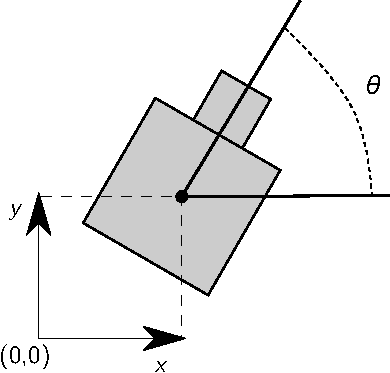
\includegraphics{figures/uav_localization.pdf}
    \caption{State representation of \gls*{uav}}
\end{figure}

To assume the first iteraction to detect the \gls*{uav} position, it's needed either to give the initial coordinates or let the algorithm detect where it might be.
The later one is less performatic due the necessity to resample the particles more times to localize its pose.

Localized the \gls*{uav}, the algorithm will verify when it'll need to resample the particles once more. This way, \emph{UpdateThreshhold} MATLAB function defines the minimum amount of change required in the three element vector to trigger the update, i.e., if \(x\), \(y\) or \(\theta\) changes by more than this minimum defined amount, an update will be triggered. The \emph{ResamplingInterval} function defines the number of updates necessary for the particle resampling, because not all variation means a real variation in the \gls*{uav} pose, they just might be some random noises.

\begin{figure}[H]
    \centering
    \begin{subfigure}{0.49\textwidth}
        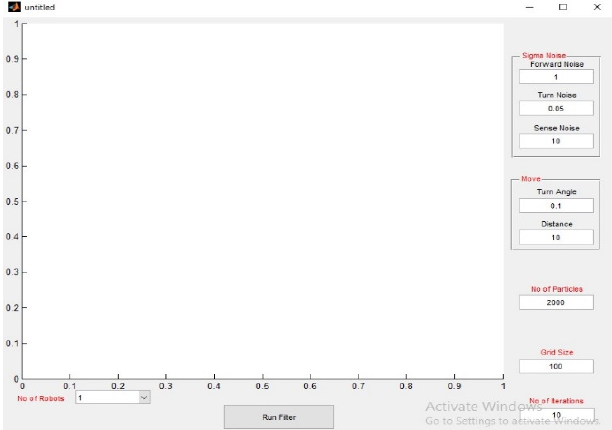
\includegraphics[width=\textwidth]{figures/gui_layout_mcl_1.png}
        \caption[GUI Layout]{GUI Layout; Source: \citet{sushant_localization_2017}}
    \end{subfigure}
    \hfill
    \begin{subfigure}{0.49\textwidth}
        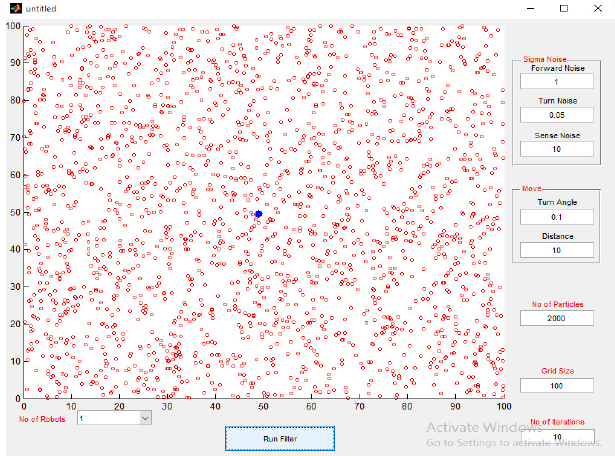
\includegraphics[width=\textwidth]{figures/gui_layout_mcl_2.png}
        \caption[First iteraction]{First iteraction; Source: \citet{sushant_localization_2017}}
    \end{subfigure}

    \begin{subfigure}{0.49\textwidth}
        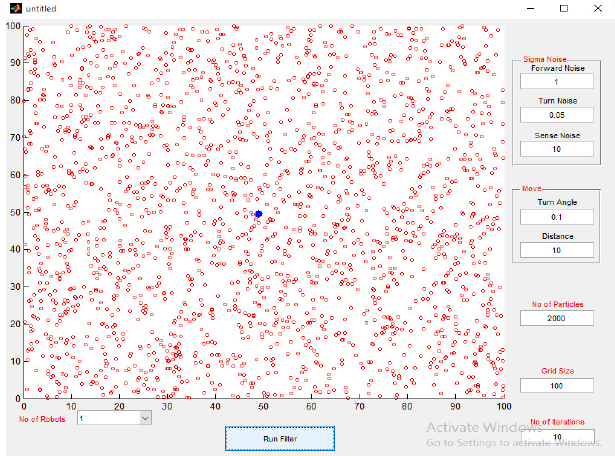
\includegraphics[width=\textwidth]{figures/gui_layout_mcl_2.png}
        \caption[Second iteraction]{Second iteraction; Source: \citet{sushant_localization_2017}}
    \end{subfigure}
    \hfill
    \begin{subfigure}{0.49\textwidth}
        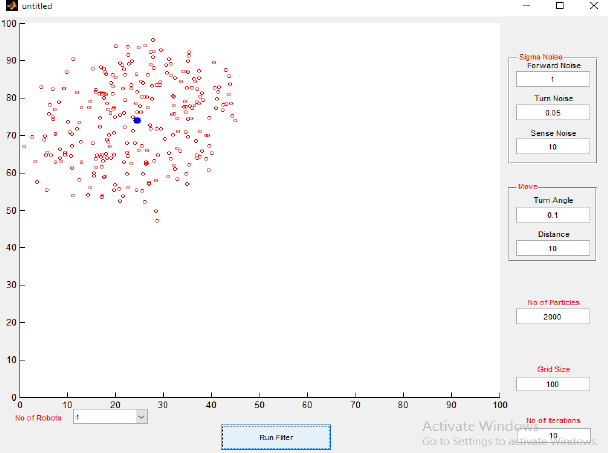
\includegraphics[width=\textwidth]{figures/gui_layout_mcl_3.png}
        \caption[Third iteraction]{Third iteraction; Source: \citet{sushant_localization_2017}}
    \end{subfigure}
    \caption{GUI interface to locate the \gls*{uav} pose.}
\end{figure}